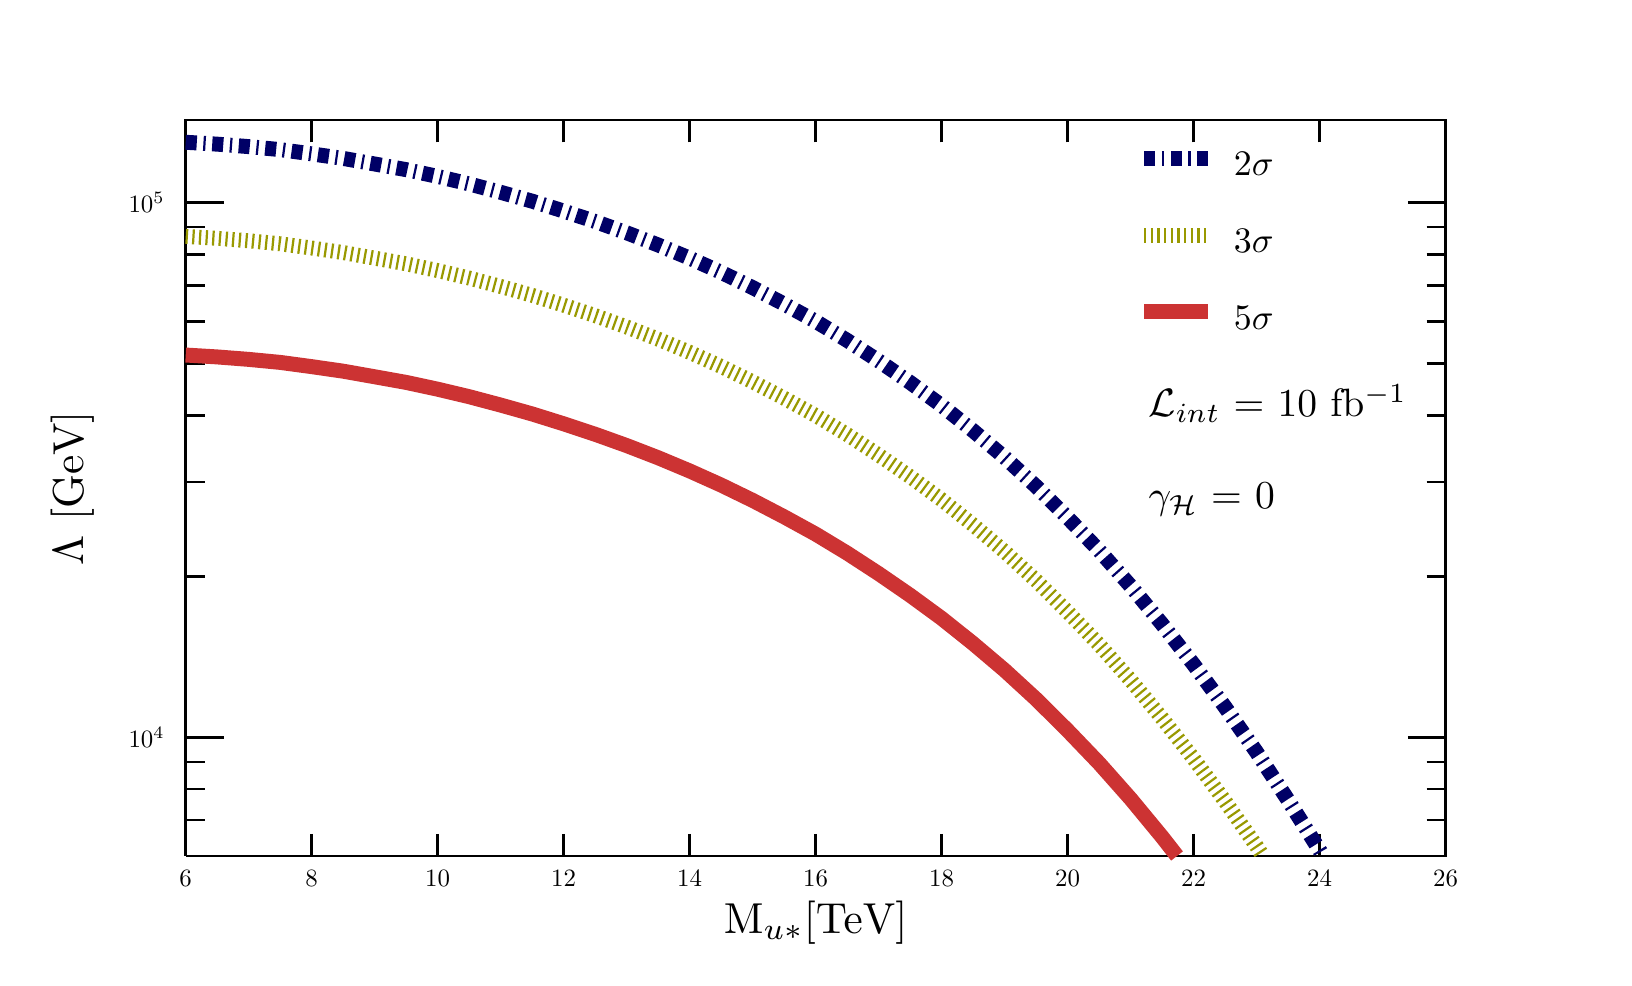
\begin{tikzpicture}
\pgfdeclareplotmark{cross} {
\pgfpathmoveto{\pgfpoint{-0.3\pgfplotmarksize}{\pgfplotmarksize}}
\pgfpathlineto{\pgfpoint{+0.3\pgfplotmarksize}{\pgfplotmarksize}}
\pgfpathlineto{\pgfpoint{+0.3\pgfplotmarksize}{0.3\pgfplotmarksize}}
\pgfpathlineto{\pgfpoint{+1\pgfplotmarksize}{0.3\pgfplotmarksize}}
\pgfpathlineto{\pgfpoint{+1\pgfplotmarksize}{-0.3\pgfplotmarksize}}
\pgfpathlineto{\pgfpoint{+0.3\pgfplotmarksize}{-0.3\pgfplotmarksize}}
\pgfpathlineto{\pgfpoint{+0.3\pgfplotmarksize}{-1.\pgfplotmarksize}}
\pgfpathlineto{\pgfpoint{-0.3\pgfplotmarksize}{-1.\pgfplotmarksize}}
\pgfpathlineto{\pgfpoint{-0.3\pgfplotmarksize}{-0.3\pgfplotmarksize}}
\pgfpathlineto{\pgfpoint{-1.\pgfplotmarksize}{-0.3\pgfplotmarksize}}
\pgfpathlineto{\pgfpoint{-1.\pgfplotmarksize}{0.3\pgfplotmarksize}}
\pgfpathlineto{\pgfpoint{-0.3\pgfplotmarksize}{0.3\pgfplotmarksize}}
\pgfpathclose
\pgfusepathqstroke
}
\pgfdeclareplotmark{cross*} {
\pgfpathmoveto{\pgfpoint{-0.3\pgfplotmarksize}{\pgfplotmarksize}}
\pgfpathlineto{\pgfpoint{+0.3\pgfplotmarksize}{\pgfplotmarksize}}
\pgfpathlineto{\pgfpoint{+0.3\pgfplotmarksize}{0.3\pgfplotmarksize}}
\pgfpathlineto{\pgfpoint{+1\pgfplotmarksize}{0.3\pgfplotmarksize}}
\pgfpathlineto{\pgfpoint{+1\pgfplotmarksize}{-0.3\pgfplotmarksize}}
\pgfpathlineto{\pgfpoint{+0.3\pgfplotmarksize}{-0.3\pgfplotmarksize}}
\pgfpathlineto{\pgfpoint{+0.3\pgfplotmarksize}{-1.\pgfplotmarksize}}
\pgfpathlineto{\pgfpoint{-0.3\pgfplotmarksize}{-1.\pgfplotmarksize}}
\pgfpathlineto{\pgfpoint{-0.3\pgfplotmarksize}{-0.3\pgfplotmarksize}}
\pgfpathlineto{\pgfpoint{-1.\pgfplotmarksize}{-0.3\pgfplotmarksize}}
\pgfpathlineto{\pgfpoint{-1.\pgfplotmarksize}{0.3\pgfplotmarksize}}
\pgfpathlineto{\pgfpoint{-0.3\pgfplotmarksize}{0.3\pgfplotmarksize}}
\pgfpathclose
\pgfusepathqfillstroke
}
\pgfdeclareplotmark{newstar} {
\pgfpathmoveto{\pgfqpoint{0pt}{\pgfplotmarksize}}
\pgfpathlineto{\pgfqpointpolar{44}{0.5\pgfplotmarksize}}
\pgfpathlineto{\pgfqpointpolar{18}{\pgfplotmarksize}}
\pgfpathlineto{\pgfqpointpolar{-20}{0.5\pgfplotmarksize}}
\pgfpathlineto{\pgfqpointpolar{-54}{\pgfplotmarksize}}
\pgfpathlineto{\pgfqpointpolar{-90}{0.5\pgfplotmarksize}}
\pgfpathlineto{\pgfqpointpolar{234}{\pgfplotmarksize}}
\pgfpathlineto{\pgfqpointpolar{198}{0.5\pgfplotmarksize}}
\pgfpathlineto{\pgfqpointpolar{162}{\pgfplotmarksize}}
\pgfpathlineto{\pgfqpointpolar{134}{0.5\pgfplotmarksize}}
\pgfpathclose
\pgfusepathqstroke
}
\pgfdeclareplotmark{newstar*} {
\pgfpathmoveto{\pgfqpoint{0pt}{\pgfplotmarksize}}
\pgfpathlineto{\pgfqpointpolar{44}{0.5\pgfplotmarksize}}
\pgfpathlineto{\pgfqpointpolar{18}{\pgfplotmarksize}}
\pgfpathlineto{\pgfqpointpolar{-20}{0.5\pgfplotmarksize}}
\pgfpathlineto{\pgfqpointpolar{-54}{\pgfplotmarksize}}
\pgfpathlineto{\pgfqpointpolar{-90}{0.5\pgfplotmarksize}}
\pgfpathlineto{\pgfqpointpolar{234}{\pgfplotmarksize}}
\pgfpathlineto{\pgfqpointpolar{198}{0.5\pgfplotmarksize}}
\pgfpathlineto{\pgfqpointpolar{162}{\pgfplotmarksize}}
\pgfpathlineto{\pgfqpointpolar{134}{0.5\pgfplotmarksize}}
\pgfpathclose
\pgfusepathqfillstroke
}
\definecolor{c}{rgb}{1,1,1};
\draw [color=c, fill=c] (0,0) rectangle (20,11.6806);
\draw [color=c, fill=c] (2,1.16806) rectangle (18,10.5125);
\definecolor{c}{rgb}{0,0,0};
\draw [c,line width=0.9] (2,1.16806) -- (2,10.5125) -- (18,10.5125) -- (18,1.16806) -- (2,1.16806);
\definecolor{c}{rgb}{1,1,1};
\draw [color=c, fill=c] (2,1.16806) rectangle (18,10.5125);
\definecolor{c}{rgb}{0,0,0};
\draw [c,line width=0.9] (2,1.16806) -- (2,10.5125) -- (18,10.5125) -- (18,1.16806) -- (2,1.16806);
\draw [c,line width=0.9] (2,1.16806) -- (18,1.16806);
\draw (10,0.327056) node[scale=1.56475, color=c, rotate=0]{M$_{u*} $[TeV]};
\draw [c,line width=0.9] (2,1.44839) -- (2,1.16806);
\draw [c,line width=0.9] (3.6,1.44839) -- (3.6,1.16806);
\draw [c,line width=0.9] (5.2,1.44839) -- (5.2,1.16806);
\draw [c,line width=0.9] (6.8,1.44839) -- (6.8,1.16806);
\draw [c,line width=0.9] (8.4,1.44839) -- (8.4,1.16806);
\draw [c,line width=0.9] (10,1.44839) -- (10,1.16806);
\draw [c,line width=0.9] (11.6,1.44839) -- (11.6,1.16806);
\draw [c,line width=0.9] (13.2,1.44839) -- (13.2,1.16806);
\draw [c,line width=0.9] (14.8,1.44839) -- (14.8,1.16806);
\draw [c,line width=0.9] (16.4,1.44839) -- (16.4,1.16806);
\draw [c,line width=0.9] (18,1.44839) -- (18,1.16806);
\draw [anchor=base] (2,0.782598) node[scale=0.900036, color=c, rotate=0]{6};
\draw [anchor=base] (3.6,0.782598) node[scale=0.900036, color=c, rotate=0]{8};
\draw [anchor=base] (5.2,0.782598) node[scale=0.900036, color=c, rotate=0]{10};
\draw [anchor=base] (6.8,0.782598) node[scale=0.900036, color=c, rotate=0]{12};
\draw [anchor=base] (8.4,0.782598) node[scale=0.900036, color=c, rotate=0]{14};
\draw [anchor=base] (10,0.782598) node[scale=0.900036, color=c, rotate=0]{16};
\draw [anchor=base] (11.6,0.782598) node[scale=0.900036, color=c, rotate=0]{18};
\draw [anchor=base] (13.2,0.782598) node[scale=0.900036, color=c, rotate=0]{20};
\draw [anchor=base] (14.8,0.782598) node[scale=0.900036, color=c, rotate=0]{22};
\draw [anchor=base] (16.4,0.782598) node[scale=0.900036, color=c, rotate=0]{24};
\draw [anchor=base] (18,0.782598) node[scale=0.900036, color=c, rotate=0]{26};
\draw [c,line width=0.9] (2,10.5125) -- (18,10.5125);
\draw [c,line width=0.9] (2,10.2322) -- (2,10.5125);
\draw [c,line width=0.9] (3.6,10.2322) -- (3.6,10.5125);
\draw [c,line width=0.9] (5.2,10.2322) -- (5.2,10.5125);
\draw [c,line width=0.9] (6.8,10.2322) -- (6.8,10.5125);
\draw [c,line width=0.9] (8.4,10.2322) -- (8.4,10.5125);
\draw [c,line width=0.9] (10,10.2322) -- (10,10.5125);
\draw [c,line width=0.9] (11.6,10.2322) -- (11.6,10.5125);
\draw [c,line width=0.9] (13.2,10.2322) -- (13.2,10.5125);
\draw [c,line width=0.9] (14.8,10.2322) -- (14.8,10.5125);
\draw [c,line width=0.9] (16.4,10.2322) -- (16.4,10.5125);
\draw [c,line width=0.9] (18,10.2322) -- (18,10.5125);
\draw [c,line width=0.9] (2,1.16806) -- (2,10.5125);
\draw (0.56,5.84029) node[scale=1.56475, color=c, rotate=90]{$\Lambda$ [GeV]};
\draw [c,line width=0.9] (2.24,1.16854) -- (2,1.16854);
\draw [c,line width=0.9] (2.24,1.62313) -- (2,1.62313);
\draw [c,line width=0.9] (2.24,2.01691) -- (2,2.01691);
\draw [c,line width=0.9] (2.24,2.36425) -- (2,2.36425);
\draw [c,line width=0.9] (2.48,2.67496) -- (2,2.67496);
\draw [anchor= east] (1.844,2.67496) node[scale=0.900036, color=c, rotate=0]{$10^{4}$};
\draw [c,line width=0.9] (2.24,4.71905) -- (2,4.71905);
\draw [c,line width=0.9] (2.24,5.91476) -- (2,5.91476);
\draw [c,line width=0.9] (2.24,6.76313) -- (2,6.76313);
\draw [c,line width=0.9] (2.24,7.42118) -- (2,7.42118);
\draw [c,line width=0.9] (2.24,7.95884) -- (2,7.95884);
\draw [c,line width=0.9] (2.24,8.41343) -- (2,8.41343);
\draw [c,line width=0.9] (2.24,8.80721) -- (2,8.80721);
\draw [c,line width=0.9] (2.24,9.15456) -- (2,9.15456);
\draw [c,line width=0.9] (2.48,9.46526) -- (2,9.46526);
\draw [anchor= east] (1.844,9.46526) node[scale=0.900036, color=c, rotate=0]{$10^{5}$};
\draw [c,line width=0.9] (18,1.16806) -- (18,10.5125);
\draw [c,line width=0.9] (17.76,1.16854) -- (18,1.16854);
\draw [c,line width=0.9] (17.76,1.62313) -- (18,1.62313);
\draw [c,line width=0.9] (17.76,2.01691) -- (18,2.01691);
\draw [c,line width=0.9] (17.76,2.36425) -- (18,2.36425);
\draw [c,line width=0.9] (17.52,2.67496) -- (18,2.67496);
\draw [c,line width=0.9] (17.76,4.71905) -- (18,4.71905);
\draw [c,line width=0.9] (17.76,5.91476) -- (18,5.91476);
\draw [c,line width=0.9] (17.76,6.76313) -- (18,6.76313);
\draw [c,line width=0.9] (17.76,7.42118) -- (18,7.42118);
\draw [c,line width=0.9] (17.76,7.95884) -- (18,7.95884);
\draw [c,line width=0.9] (17.76,8.41343) -- (18,8.41343);
\draw [c,line width=0.9] (17.76,8.80721) -- (18,8.80721);
\draw [c,line width=0.9] (17.76,9.15456) -- (18,9.15456);
\draw [c,line width=0.9] (17.52,9.46526) -- (18,9.46526);
\definecolor{c}{rgb}{0,0,0.4};
\draw [c,dash pattern=on 4.00pt off 2.40pt on 0.80pt off 2.40pt ,line width=5.4] (2,10.2322) -- (2.4,10.2082) -- (2.8,10.177) -- (3.2,10.1386) -- (3.6,10.0848) -- (4,10.0271) -- (4.4,9.95616) -- (4.8,9.88441) -- (5.2,9.79823) -- (5.6,9.70312) --
 (6,9.59665) -- (6.4,9.4839) -- (6.8,9.35877) -- (7.2,9.226) -- (7.6,9.08241) -- (8,8.9277) -- (8.4,8.76032) -- (8.8,8.58063) -- (9.2,8.38606) -- (9.6,8.17774) -- (10,7.95837) -- (10.4,7.7163) -- (10.8,7.45606) -- (11.2,7.181) -- (11.6,6.88821) --
 (12,6.56867) -- (12.4,6.2296) -- (12.8,5.86222) -- (13.2,5.46509) -- (13.6,5.04812) -- (14,4.59662) -- (14.4,4.11243) -- (14.8,3.60058) -- (15.2,3.05868) -- (15.6,2.48683) -- (16,1.87702) -- (16.4,1.24148) -- (16.4423,1.16806);
\definecolor{c}{rgb}{0.6,0.6,0};
\draw [c,dash pattern=on 0.80pt off 1.60pt ,line width=5.4] (2,9.03649) -- (2.4,9.01247) -- (2.8,8.98127) -- (3.2,8.94287) -- (3.6,8.88909) -- (4,8.83135) -- (4.4,8.76046) -- (4.8,8.6887) -- (5.2,8.60252) -- (5.6,8.50742) -- (6,8.40093) --
 (6.4,8.2882) -- (6.8,8.16306) -- (7.2,8.03029) -- (7.6,7.8867) -- (8,7.73199) -- (8.4,7.5646) -- (8.8,7.38492) -- (9.2,7.19035) -- (9.6,6.98203) -- (10,6.76266) -- (10.4,6.52059) -- (10.8,6.26035) -- (11.2,5.98529) -- (11.6,5.69251) -- (12,5.37295)
 -- (12.4,5.03389) -- (12.8,4.66651) -- (13.2,4.26938) -- (13.6,3.8524) -- (14,3.4009) -- (14.4,2.91671) -- (14.8,2.40488) -- (15.2,1.86297) -- (15.6,1.29111) -- (15.6807,1.16806);
\definecolor{c}{rgb}{0.8,0.2,0.2};
\draw [c,line width=5.4] (2,7.53007) -- (2.4,7.50605) -- (2.8,7.47485) -- (3.2,7.43646) -- (3.6,7.38268) -- (4,7.32493) -- (4.4,7.25404) -- (4.8,7.18229) -- (5.2,7.0961) -- (5.6,7.00101) -- (6,6.89451) -- (6.4,6.78178) -- (6.8,6.65664) --
 (7.2,6.52387) -- (7.6,6.38027) -- (8,6.22557) -- (8.4,6.05818) -- (8.8,5.8785) -- (9.2,5.68393) -- (9.6,5.47562) -- (10,5.25623) -- (10.4,5.01417) -- (10.8,4.75394) -- (11.2,4.47886) -- (11.6,4.18608) -- (12,3.86653) -- (12.4,3.52746) --
 (12.8,3.16009) -- (13.2,2.76297) -- (13.6,2.34598) -- (14,1.89448) -- (14.4,1.4103) -- (14.5893,1.16806);
\definecolor{c}{rgb}{0,0,0};
\draw (10,11.301) node[scale=1.2177, color=c, rotate=0]{ };
\draw [anchor=base west] (15.15,9.80681) node[scale=1.29711, color=c, rotate=0]{$2\sigma$};
\definecolor{c}{rgb}{0,0,0.4};
\draw [c,dash pattern=on 4.00pt off 2.40pt on 0.80pt off 2.40pt ,line width=5.4] (14.1725,10.0258) -- (14.9775,10.0258);
\definecolor{c}{rgb}{0,0,0};
\draw [anchor=base west] (15.15,8.83343) node[scale=1.29711, color=c, rotate=0]{$3\sigma$};
\definecolor{c}{rgb}{0.6,0.6,0};
\draw [c,dash pattern=on 0.80pt off 1.60pt ,line width=5.4] (14.1725,9.05244) -- (14.9775,9.05244);
\definecolor{c}{rgb}{0,0,0};
\draw [anchor=base west] (15.15,7.86005) node[scale=1.29711, color=c, rotate=0]{$5\sigma$};
\definecolor{c}{rgb}{0.8,0.2,0.2};
\draw [c,line width=5.4] (14.1725,8.07906) -- (14.9775,8.07906);
\definecolor{c}{rgb}{0,0,0};
\draw [anchor=base west] (14.05,6.74553) node[scale=1.42947, color=c, rotate=0]{$\mathcal{L}_{int}$ = 10 fb$^{-1}$};
\draw [anchor=base west] (14.05,5.57747) node[scale=1.42947, color=c, rotate=0]{$\gamma_{\mathcal{H}}$ = 0};
\end{tikzpicture}
